\documentclass[electronics,article,submit,pdftex,moreauthors]{Definitions/mdpi}
\usepackage{algorithm,algpseudocode}
\newcolumntype{Y}{>{\raggedright\arraybackslash}X}
\usetikzlibrary{arrows.meta,positioning}
\firstpage{1}
\pubvolume{1}\issuenum{1}\articlenumber{0}
\pubyear{2026}\copyrightyear{2026}
\datereceived{ }\daterevised{ }\dateaccepted{ }\datepublished{ }
\setlength{\headheight}{26pt}
\hreflink{https://doi.org/}
\Title{PBEA: Policy-Bound Composition of State-Transition Integrity and Runtime Confinement}
\TitleCitation{Policy-Bound Composition for Stateful Services}
\Author{SeongSu Park $^{1}$ and Ki-Hyung Kim $^{2}$}
\AuthorNames{SeongSu Park and Ki-Hyung Kim}
\AuthorCitation{Park, S.; Kim, K.}
\address{%
$^{1}$ \quad Department of Computer Engineering, Ajou University, Suwon, Republic of Korea; parky@ajou.ac.kr\\
$^{2}$ \quad Department of Cyber Security, Ajou University, Suwon, Republic of Korea; kkim86@ajou.ac.kr}
\corres{Corresponding author designation requires author confirmation before submission.}
\abstract{An authorized request can violate business invariants or exercise undeclared resources. Policy-Bound Execution Architecture (PBEA) composes candidate-state enforcement, runtime confinement, component policy identities, and explicit failure evidence. A Rust/OpenBSD implementation distinguishes application completion from supervisor-observed native termination and policy identity from actual kernel configuration. Reanalysis reproduces an archived 1,080-record four-mode corpus, which demonstrates complementary state and runtime boundaries. A separate 540-record comparison against unbound composition retains both layers while varying component identities: bound composition rejects all 120 declared mismatch trials, whereas unbound composition accepts them. Both configurations permit a deliberately mislabeled installation, establishing the limit of identity checks. Boundary tests show that allowed external transmissions can survive candidate Abort and that preopened descriptors retain authority. A new five-mode benchmark retains 150,000 raw operation timings in 300 independent process blocks across three workloads. It reports absolute and relative costs without treating within-process samples as independent experiments. The contribution is a reproducible integration contract under trusted-code and kernel assumptions, not universal attack prevention, kernel attestation, or atomic rollback of external I/O.}
\keyword{policy enforcement; state integrity; runtime confinement; OpenBSD; post-authorization control; reproducibility}
\newcommand{\EvidenceDir}{../../results/204_Astra_review/generated}
\begin{document}

\section{Introduction}\label{sec:introduction}
Zero-trust architecture strengthens decisions about access to protected resources, rather than trusting network location alone~\cite{rose2020zta,chandramouli2023zta}. An allowed request can nevertheless produce an invalid reservation, read an undeclared file, or use a stale service configuration. This paper studies the narrower execution problem: how to combine business-state checks and process resource restrictions while identifying the policy used by each component.

The problem is not that all existing systems stop at authentication. Usage control already includes ongoing decisions, mutable attributes, conditions, and obligations~\cite{park2004ucon}. System-transaction sandboxes can constrain effects spanning multiple system calls~\cite{jana2011txbox}. Capability systems and information-flow control address distinct resource and propagation questions~\cite{watson2010capsicum,krohn2007flume}. PBEA does not supersede those mechanisms. Its proposed contribution is an explicit, implementable contract linking a serial state transition, a worker-lifetime runtime plan, an effective-policy identity, and evidence whose provenance and completeness are stated.

Two distinctions are central. First, an application invariant and an operating-system capability describe different effect classes. Enabling both controls does not automatically establish that their configurations share a policy identity. Second, equality of recorded identities is not proof that a trusted mapper installed the right operating-system constraints. We separate these properties instead of crediting a digest comparison with remote attestation.

The retained evaluation comprises four configurations and nine deterministic fixtures, not a population of independent real-world attacks. A symmetric ablation shows which control supplies which property. An additional unbound-composition baseline, B3, tests the narrower identity-consistency contract while retaining both protection layers. Its separately frozen implementation produced 540 additional native records and 300 benchmark process blocks; these results are not merged into the original corpus.

The contributions are: (1) a bounded execution contract with separate application and native-failure semantics; (2) a Rust/OpenBSD mapping with worker-policy lifetime checks and explicit trusted components; and (3) reproducible effect-family and boundary evaluation, including honest accounting for missing historical timing samples. We ask whether each plane preserves its intended boundary (RQ1), which identity mismatches a bound composition can detect (RQ2), and what costs and failure boundaries the evidence actually supports (RQ3).

\section{Background and Related Work}\label{sec:related}
\subsection{Ongoing control, integrity, and contracts}
UCONABC is a close conceptual neighbor: it does not restrict authorization to an initial decision~\cite{park2004ucon}. PBEA instead chooses a concrete implementation boundary around candidate-state publication and worker-local resource confinement. It does not implement the full UCON model or show that UCON cannot express such requirements. Design by Contract makes preconditions, postconditions, and invariants explicit~\cite{meyer1992contract}; a contract alone does not mediate filesystem or network authority. Runtime monitoring also has principled limits on the policies it can enforce~\cite{schneider2000enforceable}. PBEA's endpoint check remains trusted application code, not an unbypassable kernel destination filter.

Clark--Wilson's constrained data and well-formed transactions are also a close integrity reference~\cite{clarkwilson1987integrity}. PBEA does not claim to invent application integrity policy. Its runtime plane and policy/evidence contract address a separate composition question, and a small reference implementation does not establish organizational separation-of-duty guarantees. Runtime application self-protection (RASP) is an overlapping engineering area, not a single competing algorithm. OWASP AppSensor provides application-layer detection and automated response~\cite{owaspAppSensorRevision}; PBEA evaluates a specific candidate-publication and worker-policy contract, without claiming that detection-and-response systems cannot implement comparable guards.

\subsection{Transactional sandboxes and capabilities}
TxBox uses system transactions to sandbox untrusted application effects~\cite{jana2011txbox}. This is stronger than the present implementation with respect to rollback of system resources inside a transaction. PBEA's in-memory candidate is not a system transaction: an allowed network transmission before Abort may remain visible. Capsicum reduces ambient authority through descriptor capabilities~\cite{watson2010capsicum}; PBEA's pathname restrictions do not revoke all authority in already-open descriptors. Flume governs information flow through OS abstractions~\cite{krohn2007flume}; PBEA does not claim general noninterference.

\subsection{Current enforcement research}
BeeBox hardens the BPF runtime against transient execution attacks and evaluates real BPF workloads~\cite{jin2024beebox}. Its threat and enforcement unit differ from PBEA's trusted kernel and serial application state. Such work is not an absent feature to mark as a failure in a comparison matrix. It addresses a different boundary. Supply-chain provenance, such as in-toto~\cite{torresarias2019intoto}, likewise does not make a process's domain mutation correct merely by identifying its artifacts.

\begin{table}[H]\caption{Closest approaches and the distinction investigated here. ``Outside scope'' is not evidence of inability.}\label{tab:related}
\begin{tabularx}{\textwidth}{lYYY}
\toprule Approach & Primary semantics & Resource/evidence boundary & Relation to PBEA\\\midrule
UCONABC & Ongoing authorization and mutable attributes & Model-level usage control & Broader usage model; not a measured competing implementation\\
TxBox & System-transaction policy and recovery & Kernel transaction workset & External rollback not supplied by PBEA\\
Capsicum & Capability-oriented authority & Descriptor rights and capability mode & Resource confinement, not domain-specific invariant semantics\\
Flume & Information-flow constraints & OS abstractions and labels & Noninterference differs from candidate-state validity\\
BeeBox & BPF runtime hardening & Kernel BPF execution & Kernel defense outside the present trusted-kernel model\\
PBEA & Serial domain transition plus policy identity & OpenBSD worker and local supervisor & Evaluated integration contract; no general dominance claim\\\bottomrule
\end{tabularx}\end{table}

\section{System and Threat Model}\label{sec:model}
The request $q=(a,s,c,u)$ identifies actor, asset, context, and operation. The threat begins after authenticated access is allowed. We trust the Rust verifier, policy source, resolver, runtime mapper, evidence supervisor, cryptographic primitives, kernel, and hypervisor. The adversary controls admitted request contents and, in explicit deployment-drift fixtures, the declared identities or versions supplied to independently managed components. The wrong-install counterexample deliberately violates the trusted-mapper assumption and must not be scored as an attack prevented by an identity comparison.

A worker uses one immutable runtime policy for its lifetime. Several operations may share this policy. Replacing or expanding it requires a new worker. OpenBSD restrictions are process-wide and monotonic; a request cannot restore privileges removed by an earlier pledge, nor extend a locked unveil table~\cite{openbsd79pledge,openbsd79unveil}.

Let $D_b,D_a$ be before/after committed domain state, $T_b,T_a$ be trust state, and $D^*$ be a detached candidate. For an application Commit,
\begin{equation}
I(D_b,D^*,u,c)\quad\land\quad D_a=\operatorname{install}(D^*).\label{eq:commit}
\end{equation}
For Reject or Abort, the intended domain property is $D_a=D_b$. Quarantine also leaves the candidate uninstalled but may update $T_a$ according to a separate trust-state rule. Immutable before-state hashes must be captured before mutation; a reference alias to the live state is insufficient.

Let $E^+$ denote successful observable runtime effects and $C(P_R)$ the allowed effects of the runtime policy:
\begin{equation}
\operatorname{RuntimeConform}(q,P_R)\equiv E^+(q)\subseteq C(P_R).\label{eq:runtime}
\end{equation}
A denied prohibited attempt does not violate Equation~\eqref{eq:runtime}. A counterexample to ``state integrity implies runtime conformance'' is a valid domain transition accompanied by an actually successful undeclared file read in an unconstrained execution, not merely an attempted read. Conversely, permitted resource usage can accompany a domain mutation that violates Equation~\eqref{eq:commit}.

\subsection{Identity consistency versus enforcement correctness}
An effective policy $P$ has a deterministic identifier
\begin{equation}
h_P=\operatorname{SHA256}(\operatorname{PolicyNormalize}(P)).\label{eq:policy_digest}
\end{equation}
The existing implementation sorts object members and explicitly set-like policy arrays. Ordered arrays remain ordered. This is a policy-specific normalization, not a demonstrated general RFC~8785 implementation. JCS specifies additional JSON number serialization and UTF-16 member-ordering requirements~\cite{rundgren2020jcs}; no general JCS compliance is inferred from the old golden policy digest.

For request, transition, runtime-plan, and evidence identities, define
\begin{equation}
\operatorname{IdentityConsistent}\equiv h_q=h_I=h_R=h_e.\label{eq:identity}
\end{equation}
An input failing Equation~\eqref{eq:identity} can be correctly rejected. Thus input admissibility and enforcement correctness are different predicates. The operational requirement is that a bound worker reject inconsistent identities before protected dispatch, not that every rejected request satisfy identity consistency. Even four equal identities do not attest the OS configuration: a faulty trusted mapper can install different calls while labeling them identically.

\subsection{Application and native outcomes}
Application completion has Commit, Reject, Abort, or Quarantine. StartupFailure occurs before readiness. A supervisor may instead observe native termination, with no application outcome. For such a record, the child after-state is unknown unless independently observed; an unchanged parent object is not evidence about the dead child's state. Completion evidence and termination observations therefore have separate origins and completeness flags. None implies durable storage, crash recovery, or tamper-proof distributed logging.

\section{PBEA Design}\label{sec:design}
Figure~\ref{fig:architecture} shows startup before admission. Source policy is parsed without duplicate members, schema checked, and resolved for inheritance, defaults, and conflicts. The effective policy generates a digest and a runtime plan. Resource preparation precedes listener readiness, unveil application, unveil lock, and pledge. The protected loop is entered only after installation succeeds. Endpoint allowlists are separately checked in the application before connect.

\begin{figure}[H]\centering
\begin{tikzpicture}[
  box/.style={draw,rounded corners,align=center,text width=4.1cm,minimum height=11mm,font=\small},
  arr/.style={-{Latex[length=2mm]},thick},node distance=7mm and 10mm]
\node[box,fill=gray!10] (policy) {Strict policy input\\Resolve policy parents\\and defaults};
\node[box,right=of policy,fill=gray!10] (plan) {Effective identity and runtime plan\\One immutable worker epoch};
\node[box,below=of plan,fill=green!8] (install) {Prepare resources; listener\\unveil rules; lock; pledge};
\node[box,below=of install,fill=green!8] (ready) {Ready only on successful install\\Otherwise: startup failure};
\node[box,left=of ready,fill=blue!6] (request) {Admitted request\\Check worker policy identity};
\node[box,below=of request,fill=blue!6] (candidate) {Snapshot domain and trust state\\Authorize; validate; prepare candidate};
\node[box,below=of candidate,fill=blue!6] (outcome) {Reconcile; route outcome\\Commit / Reject / Abort / Quarantine};
\node[box,right=of outcome,fill=orange!8] (evidence) {Application evidence\\Separate domain and trust hashes};
\node[box,below=of evidence,fill=orange!8] (supervisor) {Native termination: supervisor evidence\\Child state unknown unless observed};
\draw[arr] (policy)--(plan);
\draw[arr] (plan)--(install);
\draw[arr] (install)--(ready);
\draw[arr] (ready)--node[above,font=\small]{ready}(request);
\draw[arr] (request)--(candidate);
\draw[arr] (candidate)--(outcome);
\draw[arr] (outcome)--(evidence);
\draw[arr,dashed] (ready.east) -- ++(8mm,0) |- (supervisor.east);
\end{tikzpicture}

\caption{Worker-lifetime policy composition. The supervisor observation is not an application outcome. The same fragment is used by the standalone figure.}\label{fig:architecture}
\end{figure}

The runtime plan records policy identifier, epoch, backend identifier, normalized unveil rules, pledge string, lock requirement, and a plan digest. The added startup guard remembers the prepared policy digest and rejects a different policy at installation. The service emits epoch and plan identifiers on reaching readiness. These are local provenance records, not remote attestation or proof that the mapper is semantically correct.

\begin{algorithm}[H]\caption{Serial protected completion; native termination is observed externally.}\label{alg:execution}
\begin{algorithmic}[1]
\Require Ready worker, admitted $q$, committed $(D,T)$, immutable effective policy $P$
\State $D_b\gets\operatorname{ImmutableSnapshot}(D)$
\State $b_D\gets\operatorname{Hash}(D_b)$; $b_T\gets\operatorname{ImmutableHash}(T)$
\If{request or component identities disagree}
  \State \Return Evidence(Reject, $b_D$, Hash($D$), $b_T$, Hash($T$))
\EndIf
\State Authorize and validate the operation and input
\If{optional trust policy requires quarantine}
  \State Update $T$ according to that policy; do not install a domain candidate
  \State \Return Evidence(Quarantine, $b_D$, Hash($D$), $b_T$, Hash($T$))
\EndIf
\State $D^*\gets\operatorname{PrepareCandidate}(D,q)$
\If{protected preparation/reconciliation fails}
  \State \Return Evidence(Abort, $b_D$, Hash($D$), $b_T$, Hash($T$))
\EndIf
\If{$\neg I(D_b,D^*,u,c)$}
  \State \Return Evidence(Reject, $b_D$, Hash($D$), $b_T$, Hash($T$))
\EndIf
\State $D\gets\operatorname{Install}(D^*)$
\State \Return Evidence(Commit, $b_D$, Hash($D$), $b_T$, Hash($T$))
\end{algorithmic}\end{algorithm}

Algorithm~\ref{alg:execution} specifies the integration contract rather than claiming every optional policy is connected in every example. In the payment example, positive-amount validation occurs before tuple candidate creation and installation is inside reconciliation. The risk-aware core interface additionally separates read-only reconciliation from commit. The revision reservation service uses a detached state candidate and a conservation invariant. These implementation differences do not permit claiming external-I/O transactionality.

\section{Implementation}\label{sec:implementation}
The workspace retains the historical \texttt{poa-*} crate prefixes. The core owns typed transition outcomes; the protocol crate owns strict policy types, resolution, and normalization; the sandbox crate owns platform calls; the example crate owns domain hooks and orchestration. The revision does not rewrite the domain-blind core.

\begin{table}[H]\caption{Concrete enforcement mapping and trust boundaries.}\label{tab:mapping}
\begin{tabularx}{\textwidth}{lYY}
\toprule Policy element & Concrete implementation & Limit or failure rule\\\midrule
Unveil path and \texttt{r/w/x/c} & Read, write, execute, create/remove pathname rights & Directories apply to descendants; no general revocation of existing FDs\\
Empty unveil set & Mask root, then lock & Lock alone does not establish deny-all\\
Lock requirement & \texttt{unveil(NULL,NULL)} after rules & Failure prevents readiness\\
Pledge promises & Validated, sorted promise string & Process-wide syscall classes, not destinations\\
Network endpoints & Application IP/port/protocol predicate & Trusted check; raw socket code could bypass it\\
Policy epoch & One effective policy per worker & New policy requires new worker\\
Prepared policy & Digest compared before install & Detects declared skew, not dishonest installation metadata\\
Evidence & Application or supervisor writer & Child state can be unobserved\\\bottomrule
\end{tabularx}\end{table}

Strict parsing now rejects duplicate members before deserialization loses them. Tests cover nested duplicates, trailing input, invalid numeric/Unicode encodings, ordered-array preservation, set-like-array order invariance, and preserving distinct Unicode sequences. Existing schema, inheritance conflict, privilege-expansion, and golden digest regressions are retained. This is a restricted implementation profile; unsupported JSON semantics must not be silently called universal canonicalization.

The service opens its audit descriptor and listener before confinement. This is intentional but security-relevant: pathname visibility is not an exhaustive descriptor capability inventory. The additional FD fixture opens a synthetic outside file before installing restrictions, then compares descriptor use with a new pathname open. The current worker does not promise a complete inherited-descriptor sanitizer. Allowed child execution after exec is not evaluated; the exec-denial result does not prove safe post-exec privilege inheritance.

The reservation service starts with ten units, tracks availability and a reservation map, and enforces $available+\sum reserved=total$. It rejects duplicate reservation IDs, zero quantities, insufficient stock, and cancellation of unknown IDs. Its sequence includes normal reservation, oversubscription, duplicate input, candidate Abort, cancellation, and repeated cancellation. It is serial and in memory. No serializability theorem, persistent quarantine, OS-crash rollback, or distributed transaction is claimed.

\section{Evaluation Methodology}\label{sec:method}
\subsection{Preserved historical corpus}
The frozen evaluation source is \nolinkurl{62229cd31ad1915cdd850fe3cfd670cddf208d0c}; the reporting correction is \nolinkurl{f2be0bfbcbf2aad093018d69e513cc61b169e5e3}. The original three manuscript inputs are hash-preserved. Four raw JSONL files contain $4\times9\times30=1080$ records. The reanalysis reproduces the canonical metrics and verifies all 37 files of the retained manifest after mapping relocated paths.

B0 performs direct mutation after admitted access; B1 adds transition and digest checks; B2 installs runtime confinement without the transition guard; P combines them. B0 is not representative of every ZTA or UCON implementation. S0 is benign; S1 violates a positive-amount invariant; S2--S4 test file read, helper execution, and a controlled prohibited endpoint; S5 alternates malformed policy and missing resource; S6 repeats a wrong-digest request; S7 injects a candidate-stage fault where that stage exists; S8 changes the request digest.

S7 is N/A in B0/B2: the direct-mutation path does not execute the after-candidate fault. Its normal state change is neither a rollback failure nor a malicious effect. B1/P abort without installing the candidate. S5 is reported as separate 15-run causes rather than an undifferentiated 30-case probability.

The archived S3 supervisor spawns an isolated child that installs restrictions and attempts helper execution. The supervisor records signal and marker presence. Its local parent-domain hashes must not be interpreted as child-state after-images. An additive observation view retains original record IDs while marking the application outcome and child after-state unobserved for native termination.

\subsection{Unbound composition and additional boundaries}
B3 retains transition checks and the same runtime backend but manages component identities independently. P applies the equality contract before dispatch. Prespecified cases include aligned identities, runtime epoch skew, stale evidence identity, resolved-policy drift, request/worker epoch mismatch, and equal IDs with intentionally wrong installation. The last case tests the limitation of metadata consistency, not a property the design is expected to enforce.

Additional cases test an allowed receiver-visible transmission followed by candidate Abort, authority retained by a preopened descriptor, and the reservation sequence. The supervisor retains child failures instead of dropping them. The new validator checks completeness, uniqueness, provenance, and field consistency; an observed security failure is valid data, not grounds to reject a record. The prespecified 9 cases $\times$ 2 modes $\times$ 30 repeats produced 540 observed records. This modest integration comparison does not make B3 representative of all independently managed security systems.

\subsection{Performance and experimental units}
The historical S0 benchmark ran 100 warm-up and 5000 measured operations per mode in a long-lived process. It retained aggregate latency statistics, not individual timings. Its functional-equivalence artifact compares operation, normal result, and a normalized success label; it is not a wire-byte equivalence test. The original direct path performs a map insertion, whereas guarded paths additionally parse and validate the request and generate security evidence. Therefore their cost difference includes security-specific work.

The revision runner stores raw nanosecond samples, empty-timer measurements, a rotating mode order, and 20 independent process blocks per mode/workload. Each block warms up 100 operations and measures 500. Workloads include one asset, 128 assets, and a permitted file read. Sequential samples within a block are not independent experimental units. Quantiles and block-median ranges are reported separately. Neither throughput nor memory scaling is inferred without measurement; the payment candidate remains a tuple rather than a whole-state copy.

\section{Results}\label{sec:results}
\subsection{Reproduced effect-family results}
Table~\ref{tab:security} is generated from the revalidated historical corpus. It supports complementary protection boundaries, not a population-level attack success estimate. Transition-only prevents the tested S1 effect but not S2--S4; Runtime-only does the reverse. Full-PBEA combines them in the evaluated fixture. S5's split shows why parsing and runtime-resource readiness are not interchangeable.
\begin{table}[H]\caption{Historical results, as numerator/denominator. N/A excludes an absent fault point.}\label{tab:security}\centering
\input{\EvidenceDir/historical_security.tex}
\end{table}

Across the 90 P S2--S4 attempts, no prohibited effect succeeded. Filesystem denial, helper termination, and application endpoint rejection are distinct observations. The endpoint result is not evidence that pledge filters a destination IP. BT1 permits delivery to the explicitly allowed endpoint. BT2 denies the tested symlink traversal in B2/P, but does not establish a general race-free filesystem theorem. Repetitions demonstrate stability of these deterministic tests, not 1080 unique attack inputs.

\subsection{Historical cost and unavailable uncertainty}
Table~\ref{tab:performance} regenerates the archived steady-state summaries and derives both absolute increment and ratio. Full-PBEA's median is below one millisecond yet approximately 264.28 times the small direct-insertion baseline. Both observations matter. P being faster than B1 in this one schedule does not show that confinement improves speed.
\begin{table}[H]\caption{Historical synthetic S0 summaries in microseconds; new independent-block measurements are a separate corpus.}\label{tab:performance}\centering
\input{\EvidenceDir/historical_performance.tex}
\end{table}

B0 and B2 have identical reported P50/P95 values (0.700/0.701 microseconds) after restrictions were installed. This shows no measurable difference on the synthetic, nearly syscall-free path at the reported resolution; it says nothing about zero cost for real I/O. The missing historical sample series prevents reconstructing block uncertainty or independently checking the original quantiles. The archived startup corpus contains 30 observations per mode, with medians approximately 44 ms. No startup ranking is claimed.

\subsection{Additive native results}
\begin{table}[H]\caption{Additional B3/P observations from the separately frozen revision source.}\centering\input{\EvidenceDir/binding_results.tex}\end{table}
For aligned policies both modes committed 30/30 requests. Across the four declared mismatch cases, B3 committed all 120 and P rejected all 120 before dispatch. This supports detection of supplied identity skew, not discovery of arbitrary semantic policy drift. In the intentionally wrong-install case, both modes completed all 30 forbidden outside-file reads despite equal claimed IDs. This observed counterexample is retained, narrowing the claim to identity consistency under trusted mapping.

For allowed-send-before-Abort, the receiving socket observed all 30 transmissions per mode while the candidate domain state remained uninstalled. For the preopened descriptor fixture, both modes read the file through the existing handle in all 30 trials, while a new pathname read was denied. The reservation sequence preserved its conservation invariant and expected operation sequence in all 30 trials per mode. These outcomes distinguish transaction publication, external effects, and descriptor authority.

The new performance corpus contains 20 independent processes for each of five modes and three workloads. Table~\ref{tab:native_performance} reports pooled descriptive quantiles, not independent-sample uncertainty. For the one-asset path, P's process-block medians ranged from 186.595 to 232.644 microseconds. The corresponding ranges overlap those of B1/B3; no speedup caused by confinement is inferred. The full block statistics and empty-timer observations remain in the canonical JSON artifact.
\begin{table}[H]\caption{New native timing summaries in microseconds, generated from raw samples. Each row represents 20 independent process blocks and 10,000 measured sequential operations.}\label{tab:native_performance}\centering
\input{\EvidenceDir/native_performance.tex}
\end{table}

\section{Discussion and Limitations}\label{sec:discussion}
\subsection{What policy binding adds}
The implemented contract can detect declared disagreement between component identities and a policy change between resource preparation and installation. It cannot independently attest that trusted code used the intended system calls. B3 testing is therefore a test of deployment identity consistency under specified skew, not proof of a universal new principle. If independently managed layers carry consistent identities, B3 and P should have the same benign outcome. The architecture's novelty is bounded integration and traceability, not the discovery that two security layers can be composed.

\subsection{State, external effects, and failures}
Rejecting a candidate is not rollback of the entire service environment. An allowed send can reach a receiver before a later failure, and a descriptor opened before confinement may retain authority. External-effect buffering, outboxes, compensation, persistent state, and restart recovery would need separate implementation and evaluation. The relevant failure models are ordinary function error, child termination, service death, and OS crash; only the measured model can be credited.

\subsection{Threats to validity}
The historical experiment uses one OpenBSD 7.9 VM and a small payment fixture. Workload representativeness, privilege-authoring quality, hidden library authority, inherited descriptors, mapper correctness, and audit durability remain limits. B0/B1/B2 are chosen configurations, not commercial systems. No Linux backend claim follows from a compiling placeholder. RiskEvidence is optional, and the payment example's repeated-violation counter is not a persistent distributed quarantine service. A trusted supervisor can misreport; its evidence is not a cryptographic attestation chain.

The revised tests expand distinct causes and business sequencing, not merely repetitions. Nonetheless they remain controlled mechanism tests. A 30/30 result is not a probability bound over real attacks, even if a binomial interval can be mechanically calculated. No claim about prompt injection, arbitrary malware, malicious administrators, or compromised kernels is supported.

\begin{table}[H]\caption{Claim--evidence boundaries.}\label{tab:claims}
\begin{tabularx}{\textwidth}{YYY}
\toprule Claim & Evidence location & Restriction\\\midrule
Protected domain publication & S1, applicable S7; reservation unit test & Serial memory, no external-I/O rollback\\
Prohibited capabilities contained & Historical S2--S4 and native errno/signal & App endpoint check is TCB\\
Policy identity consistency & Worker startup guard and binding tests & No attestation of actual kernel plan\\
Normal behavior preserved & S0 hashes and normalized success & Not identical wire response payloads\\
Quantified implementation cost & Archived summaries; separate new raw blocks & Historical sample-level uncertainty unavailable\\\bottomrule
\end{tabularx}\end{table}

\section{Conclusions}\label{sec:conclusion}
PBEA specifies how a serial stateful service can combine candidate-state integrity, process resource confinement, policy identity, and explicit evidence semantics. The retained four-mode corpus supports distinct, non-substitutable enforcement roles in its fixtures. The revision narrows identity claims, distinguishes native termination from application completion, and makes the worker lifetime explicit. It also exposes the limits of domain-state rollback and historical performance data. The intended result is an auditable implementation contract and reproducible bounded evaluation, not universal prevention or superiority over existing usage control, capability, or transactional systems.

\authorcontributions{Author-specific CRediT roles and final approval must be confirmed by the authors before submission.}
\funding{The original draft reports IITP/ITRC support, grant IITP-2026-RS-2021-II211835. The authors must confirm the funding statement for the submission version.}
\institutionalreview{Not applicable to the synthetic software fixtures described here; author confirmation is required for final submission.}
\informedconsent{Not applicable to the synthetic software fixtures described here.}
\dataavailability{Historical raw evidence and newly generated local revision artifacts are retained in the project evidence package. A public archival release of this revision has not been verified. The authors must provide a reviewer-accessible release before submission. This study created and analyzed data; data sharing is not inapplicable.}
\acknowledgments{Generative AI agents assisted code, analysis, and manuscript revision. Exact tool/version disclosures and author responsibility statements require author review before submission.}
\conflictsofinterest{The authors must confirm their conflicts-of-interest declaration before submission.}
\reftitle{References}
\bibliography{month_strings,../references,revision_references}
\PublishersNote{}
\end{document}
